%%%%%%%%%%%%%%%%%%%%%%%%%%%%%%%%%%%%%%%%%%%%%%%%%%%%%%%%%%%%%%%%%%%%%%%%%%%%%%%%
%2345678901234567890123456789012345678901234567890123456789012345678901234567890
%        1         2         3         4         5         6         7         8

%\documentclass[letterpaper, 10 pt, conference]{orbieeeconfpre}  % Comment this line out if you need a4paper

\documentclass[a4paper, 10pt, journal]{wissarbIEEE}      % Use this line for a4 paper
%\conference{IEEE Conference for Awesome ORB Research}

\bibliographystyle{orbref-num}

\overrideIEEEmargins                                      % Needed to meet printer requirements.

% See the \addtolength command later in the file to balance the column lengths
% on the last page of the document

\usepackage{hyperref}
\usepackage{graphicx}
\usepackage{tabularx}
\usepackage{booktabs}
\usepackage{lipsum}

\title{\LARGE \bf Scientific Work Short Paper \\Feasibility Study - SmartWarehouse}

\author{Felix Hausberger and Robin Kuck}

\begin{document}

\maketitle

%%%%%%%%%%%%%%%%%%%%%%%%%%%%%%%%%%%%%%%%%%%%%%%%%%%%%%%%%%%%%%%%%%%%%%%%%%%%%%%%
\begin{abstract}

In this short paper the object detectors \textit{You Only Look Once} and \textit{Single Shot MultiBox Detector} are compared for precision, reactivity, training and inference behaviour and examined for their potential for industrial use. The background scenario of the Smart Warehouse offers live video data of a drone with goods in a warehouse, which are to be classffied and localized in real time. In the future, this should make it possible to carry out inventories and inventory analyses of a warehouse in a time- and cost-efficient manner conserving resources.

The goal of this feasibility study is to find out whether the Smart Warehouse scenario is technically feasible. In addition, the focus is also on the object detectors themselves, their differences in architecture, behavior and how well they are generally suitable for industrial application scenarios.

\end{abstract}

%%%%%%%%%%%%%%%%%%%%%%%%%%%%%%%%%%%%%%%%%%%%%%%%%%%%%%%%%%%%%%%%%%%%%%%%%%%%%%%%
\section{Introduction}

Object detection represents a major field of study in industrial fields like autonomous driving, industrial processing or even government monitoring. Especially in times of the industrial change towards Industry 4.0 such object detectors represent an optimization potential not to be neglected, e.g. in warehousing and logistics. Combined with an autonomous drone, such object detectors could make it possible to conduct inventory checks in a warehouse without human assistance. How different object detectors behave when applied to a real time industry scenario like \textit{SmartWarehouse} should be evaluated in this short paper. As being a feasibility study, the main goal of this work also is to discuss the feasibility of the \textit{SmartWarehouse} idea based on the performance of the two selected object detectors \textit{You Only Look Once} (YOLO) and \textit{Single Shot MultiBox Detector} (SSD) in terms of precision, responsiveness, training and inference behavior. In \autoref{relatedwork} related work to similar industry scenarios should be introduced before explaining the approach and architecture of the \textit{SmartWarehouse} prototype in \autoref{architecture}. In \autoref{evaluation} the results of the feasibility study will be presented and evaluated before the interpretability of the results is discussed in \autoref{results}. \autoref{conclusion} gives a quick coonclusion about the main achievements of this short paper.

\section{Related Work} \label{relatedwork}

The idea of automized inventory checks with drones is not new. \cite{doks.innovationGmbH.2020} uses a similar approach, but uses normal RFID technology or simple barcodes to identify a product. Using this approach only a small number of instances at a time can be identified, while using object detection algorithms enable many-numbered and faster processing. 

The paper \cite{WeiLiuDragomirAnguelovDumitruErhanChristianSzegedyScottReedChengYangFuAlexander.2016} introduces the \textit{Single Shot MultiBox Detector} (SSD), an object detector reaching up to 76.9\% mean average precision (mAP) while still keeping real time detection characteristics compared to its preceeding competitors like regional convolutional neural networks (R-CNNs). It uses a single neural network to detect objects and creates a set of default bounding boxes over different aspect ratios and scales for each feature map location instead of using an additional bounding box proposal step. 

The \textit{You only Look Once} (YOLO) algorithm was introduced in \cite{JosephRedmonSantoshDivvalaRossGirshickAliFarhadi.2016} and as well uses a single neural network to predict bounding boxes and class probabilities. Incremental improvements led to version three of YOLO, which is equally accurate as SSD, but three times faster \cite{JosephRedmon.2018}. 

\section{Architecture of the SmartWarehouse scenario} \label{architecture}

\subsection{Defining the scenario}

Two goals were defined for the feasibility study of \textit{SmartWarehouse}. First it is to be evaluated, how well existing object detectors perform in industry scenarios taking the example of \textit{SmartWarehouse} and the two object detectors YOLO and SSD. Second, one should deal with the feasibility of the implementation of this \textit{SmartWarehouse} scenario, which comprises the execution of an inventory for department stores with a drone. 

\subsection{Dataset}

The \textit{SmartWarehouse} is based on a large department store, where products are not packed in
are not packed in cartons, but are arranged as a whole on shelves. In the construction of the training data set, however, the feasibility study does not aim to represent such a store completely in the data set, but rather to select a dataset that is as extensive as possible in order to prove the general feasibility of the \textit{SmartWarehouse} scenario. In the context, the focus was therefore on beverage bottles of a department store. Nine categories were defined: \textit{Saskia Water Small}, \textit{Saskia Water Large}, \textit{Pepsi Cola Small}, \textit{Pepsi Cola Large}, \textit{ISO}, \textit{ACE}, \textit{Stenger Blackcurrant Spritzer}, \textit{Stenger Apple Spritzer}, and \textit{Vitamalz Malt Beer}. All classes are distributed equally in the data set. The data set itself is 1.45 GB big and consists of 1088 manually annotated images of resolution 2112x4608 and 24 bit color depth. The annotations are given in \textit{PascalVOC} and \textit{YOLO} format. 75\% of the images include a single instances of a beverage bottle to better train the patterns of the different classes. Furthermore, 13\% of the images contain occlusions of objects to be detected, detection situations from extreme viewing positions are represented to 4\%, and difficult illumination and lighting conditions are included to 8\%. Only a few examples (2\%) are related to different distances during detection. Care was also taken to continuously vary the backgrounds of the objects being detected. With the enrichment of the data set with representations of such difficult recording circumstances, it is hoped to increase the generalization capability of Deep Learning models based on them. Finally, to simulate the department store where several objects are to be detected at once, in 12.5\% of all images the objects are arranged on shelves, one behind the other or in beverage crates. From the total dataset of 1088 images, 90 images were extracted for later validation. The remaining 998 consist of 200 images of test data and 798 images for training. In 90\% of all images, only objects of one class are shown, since commodity inventories are likewise mostly grouped by commodity. The dataset was published on Kaggle\footnote{see \url{https://www.kaggle.com/fidsusj/smartwarehousessd} and \url{https://www.kaggle.com/fidsusj/smartwarehouseyolo}} for both PascalVOC format and YOLO format.

\subsection{Introduction of evaluation criteria}

To better compare object detectors with each other the following evaluation criteria have been defined:

\begin{itemize}
	\item Precision: The precision of an object detector measured in mAP
	\item Reactivity: The inference rate with the model measured in \textit{Frames Per Second} (FPS)
	\item Training behavior: The speed of the gradient curve until convergence measured in training epochs
	\item Inference behavior: The inference behavior under special lighting conditions, extreme viewing positions, occultation of objects, and the behavior with double detected objects measured with good, medium, poor. 
\end{itemize}

\subsection{Selection of object detectors}

For the smart warehouse scenario, a choice should be made between the four detectors Faster R-CNN, Mask R-CNN, SSD and YOLO. 

\begin{figure}[h]
	\centering
	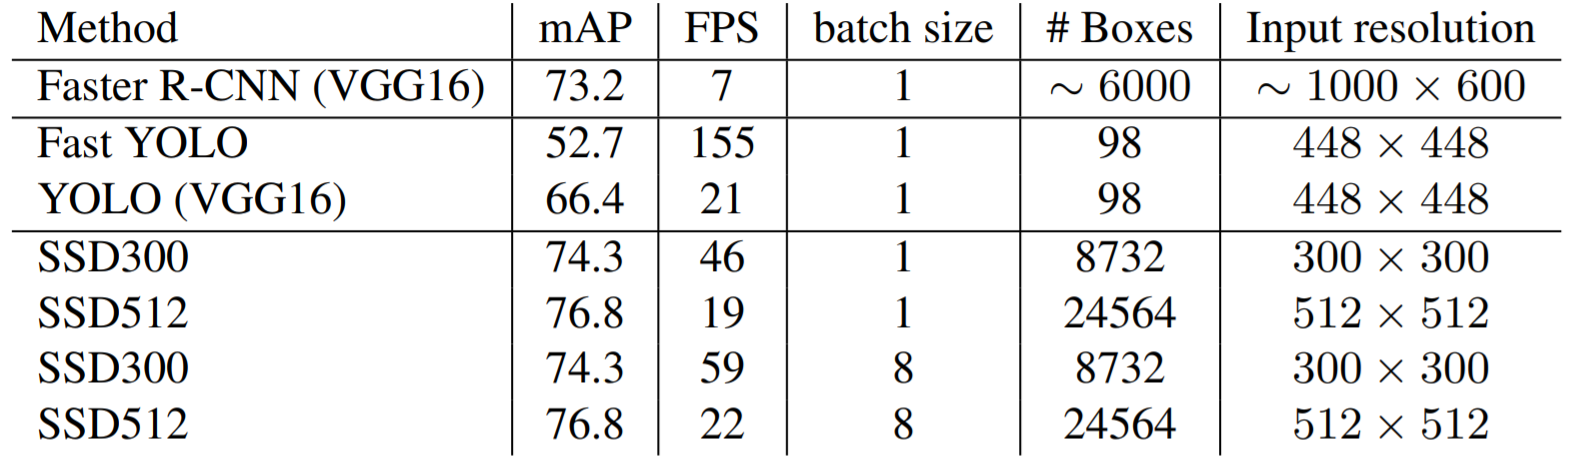
\includegraphics[width=0.5\textwidth]{fig/ssd_results.png}
	\caption{Comparison of SSD on PascalVOC 2007 \cite{WeiLiuDragomirAnguelovDumitruErhanChristianSzegedyScottReedChengYangFuAlexander.2016}}
	\label{ssd_results}
\end{figure}

According to the reference results in \autoref{ssd_results}, it is clear that the SSD performs best in terms of mAP with 74.3\% and 76.8\%, respectively. Faster-RCNN can keep up with 73.2\% in terms of mAP,
but with only 7 FPS it is not designed for fast inference. YOLO scores worse than the SSD in both categories, it essentially achieves an mAP of 66.4\% and a frame rate of 21 FPS. The SSD thus manages to maintain a good balance between precision and responsiveness. Comparing Mask-RCNN from the original paper in \cite{KaimingHeGeorgiaGkioxariPiotrDollarRossGirshick.2018} with Faster-RCNN (RoI-Align) results in a mAP difference of 38.2\% to 37.3\%. Only 5 FPS could be reached. 

To find two suitable object detectors to evaluate, the effort setup the implementations and to adapt them to be trained with a custom data set was also taken into account. Whereas the SSD and YOLO implementations were easy to handle regarding these two tasks, implementations of ferster-RCNN or Mask-RCNN were either not supported on the operating system of choice or already depricated and no longer supported. 

Due to these circumstances and the poorer performance in time-critical model inference, YOLO and SSD were selected as the two detectors to evaluate the capability of object detectors for industrial use using the smart warehouse scenario as an example. The official implementation of YOLOv3 in the \textit{Darknet} framework and a custom implementation of SSD300 in the \textit{PyTorch} framework is used.

\subsection{Drone}

Analysiert man den Markt auf programmierbare Drohnen mit einem frei zugänglichen
Software Development Kit (SDK) und integrierter Kamera, so fällt das Angebot sehr
gering aus. Im Folgenden soll ein Überblick über die zwei verfügbaren Modelle Ryze
Tech Tello EDU und Parrot Bebop 2 gegeben werden [45, 46]. 

\subsection{Training infrastructure}

Deep Lerning: Tensor operations like matrix multiplications, covolutions, ...
Needs high parallelisation and tact frequencies
GPUs: CUDA (Compute UnifiedDevice Architecture) programming model and parallel computing platform => calc operations auf GPUs auslagern

Das CUDA Toolkit beinhaltet
GPU beschleunigte Bibliotheken, einen Compiler, Entwicklungswerkzeuge sowie die
eigentliche CUDA Laufzeit und wird von vielen Deep Learning Bibliotheken genutzt,
wie z.B. PyTorch

Auch bietet NVIDIA die sogenannte NVIDIA CUDA Deep
Neural Network Library (cuDNN) an, die hardwareoptimierte Routinen zu beispielsweise
Konvolution oder Pooling ermöglicht [30]. Hauptvergleichskriterien zwischen GPUs
sind hierbei der Grad der möglichen Parallelisierung und die reine Rechenleistung im
Verhältnis zum Stromverbrauch.

AWS SageMaker, Google Cloud Platfrom AI Platform (TPUs!), Colab, Azure, FloydHub

\section{Results and evaluation} \label{evaluation}

\section{Discussion} \label{results}

\section{Conclusion} \label{conclusion}

\bibliography{mybibfile}

\end{document}
